\documentclass{beamer}
\usepackage[utf8]{inputenc}

\usetheme{Madrid}
\usecolortheme{default}
\usepackage{amsmath,amssymb,amsfonts,amsthm}
\usepackage{txfonts}
\usepackage{tkz-euclide}
\usepackage{listings}
\usepackage{adjustbox}
\usepackage{array}
\usepackage{tabularx}
\usepackage{gvv}
\usepackage{lmodern}
\usepackage{circuitikz}
\usepackage{tikz}
\usepackage{graphicx}
\usepackage{multicol}
\setbeamertemplate{page number in head/foot}[totalframenumber]

\usepackage{tcolorbox}
\tcbuselibrary{minted,breakable,xparse,skins}

\definecolor{bg}{gray}{0.95}
\DeclareTCBListing{mintedbox}{O{}m!O{}}{%
	breakable=true,
	listing engine=minted,
	listing only,
	minted language=#2,
	minted style=default,
	minted options={%
		linenos,
		gobble=0,
		breaklines=true,
		breakafter=,,
		fontsize=\small,
		numbersep=8pt,
		#1},
	boxsep=0pt,
	left skip=0pt,
	right skip=0pt,
	left=25pt,
	right=0pt,
	top=3pt,
	bottom=3pt,
	arc=5pt,
	leftrule=0pt,
	rightrule=0pt,
	bottomrule=2pt,
	toprule=2pt,
	colback=bg,
	colframe=orange!70,
	enhanced,
	overlay={%
		\begin{tcbclipinterior}
			\fill[orange!20!white] (frame.south west) rectangle ([xshift=20pt]frame.north west);
	\end{tcbclipinterior}},
}

\lstset{
	language=C,
	basicstyle=\ttfamily\small,
	keywordstyle=\color{blue},
	stringstyle=\color{orange},
	commentstyle=\color{green!60!black},
	numbers=left,
	numberstyle=\tiny\color{gray},
	breaklines=true,
	showstringspaces=false,
}

%------------------------------------------------------------
\title{1.1.47}
\author{RAVULA SHASHANK REDDY - EE25BTECH11047}
\date{}
\begin{document}

\frame{\titlepage}

\begin{frame}{Problem}

A feedback control system with high gain $K$ is shown.
\begin{figure}
    \centering
    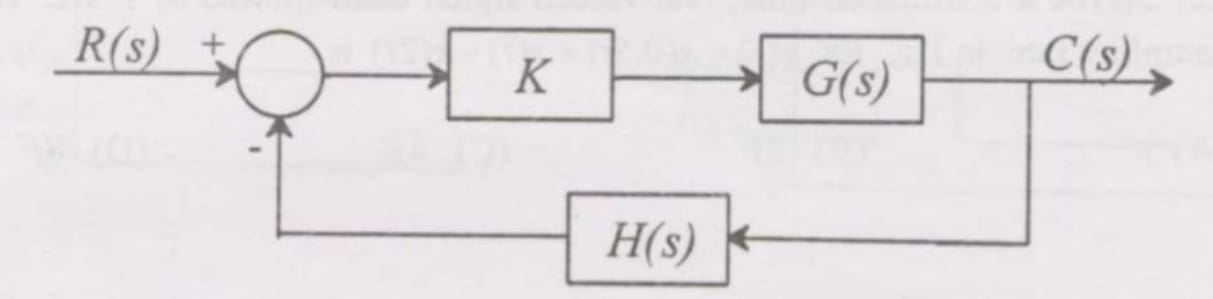
\includegraphics[width=1.0\linewidth]{fig1.jpeg}
    \caption{}
    \label{fig:placeholder}
\end{figure}
The closed loop transfer function is :

\begin{enumerate}
    \item sensitive to perturbations in $G(s)$ and $H(s)$
    \item sensitive to perturbations in $G(s)$ but not to perturbations in $H(s)$
    \item sensitive to perturbations in $H(s)$ but not to perturbations in $G(s)$
    \item insensitive to perturbations in $G(s)$ and $H(s)$
\end{enumerate}

\end{frame}

%------------------------------------------------

\begin{frame}{System Description}
R(s) $\Rightarrow$ Input  \\
C(s) $\Rightarrow$ Output \\
T(s) $\Rightarrow$ closed loop transfer function \\


The system contain the following gains:
\begin{itemize}
    \item Forward path: $K G(s)$ 
    \item Negative Feedback path: $H(s)$
\end{itemize}
\end{frame}
\begin{frame}{Solution}
At the summing junction  

\begin{align}
E(s) = R(s) - [H(s)]C(s)
\end{align}

So, now E(s) goes through the system

\begin{align}
C(s) &= [K G(s)] E(s) \\
     &= K G(s)\left[R(s) - H(s)C(s)\right]
\end{align}
\end{frame}
%------------------------------------------------

\begin{frame}{Simplification}
\begin{align}
C(s) &= K G(s)R(s) - K G(s)H(s)C(s) 
\end{align}
\begin{align}
C(s) + [K G(s)]H(s)C(s) &= K G(s)R(s) 
\end{align}
\begin{align}
C(s)\left[1 + K G(s)H(s)\right] &= K G(s)R(s)
\end{align}
\end{frame}

%------------------------------------------------

\begin{frame}{Transfer Function}
\begin{align}
T(s) = \frac{C(s)}{R(s)} = \frac{K G(s)}{1 + K G(s)H(s)}
\end{align}

\begin{align}
T(s) &= \frac{G(s)}{\frac{1}{K} + G(s)H(s)} \\
\text{As K is very large}\\
T(s) &\approx\frac{G(s)}{G(s)H(s)}\\
\quad T(s) &\approx \frac{1}{H(s)}
\end{align}
\end{frame}

%------------------------------------------------

\begin{frame}{Sensitivity Analysis}
\begin{itemize}
    \item $G(s)$ cancels out $\Rightarrow$ insensitive to $G(s)$
    \item Output depends on $H(s)$
    \item Sensitive to perturbations in $H(s)$
\end{itemize}
\end{frame}

%------------------------------------------------

\begin{frame}{Final Answer}
\begin{align}
\boxed{\text{Sensitive to perturbations in } H(s)\text{ but not in } G(s)}
\end{align}
\end{frame}

%------------------------------------------------
\begin{frame}[fragile]
\frametitle{Python Code 1}
\begin{lstlisting}
    import numpy as np
import matplotlib.pyplot as plt

w = np.linspace(0.1, 10, 500)
s = 1j * w

K = 1e5  # very large gain

# Fixed G(s)
G = 1 / (s + 1)

# Strongly different H(s)
H1 = 1 / (s + 2)
H2 = 5 / (s + 0.2)

# Closed-loop transfer functions
T1 = (K * G) / (1 + K * G * H1)
T2 = (K * G) / (1 + K * G * H2)
\end{lstlisting}
    
\end{frame}
\begin{frame}[fragile]
\frametitle{Python Code 1}
\begin{lstlisting}
# Plot H(s)
plt.figure()
plt.plot(w, abs(H1), label="H1 = 1/(s+2)")
plt.plot(w, abs(H2), '--', label="H2 = 5/(s+0.2)")
plt.title("Large Difference in H(s)")
plt.legend()
plt.grid()
plt.show()

# Plot T(s)
plt.figure()
plt.plot(w, abs(T1), label="T with H1")
plt.plot(w, abs(T2), '--', label="T with H2")
plt.title("Closed-loop T(s) (Clearly Different!)")
plt.legend()
plt.grid()
plt.show()
\end{lstlisting}
    
\end{frame}
\begin{frame}[fragile]
\frametitle{Python Code 2}
\begin{lstlisting}
import numpy as np
import matplotlib.pyplot as plt

w = np.linspace(0.1, 10, 500)
s = 1j * w

K = 1e5  # large gain

# Fixed H(s)
H = 1 / (s + 2)

# Strongly different G(s)
G1 = 1 / (s + 1)
G2 = 5 / (s + 0.2)

# Closed-loop
T1 = (K * G1) / (1 + K * G1 * H)
T2 = (K * G2) / (1 + K * G2 * H)
\end{lstlisting}
    
\end{frame}
\begin{frame}[fragile]
\frametitle{Python Code 2}
\begin{lstlisting}
# Plot G(s)
plt.figure()
plt.plot(w, abs(G1), label="G1 = 1/(s+1)")
plt.plot(w, abs(G2), '--', label="G2 = 5/(s+0.2)")
plt.title("Large Difference in G(s)")
plt.legend()
plt.grid()
plt.show()

# Plot T(s)
plt.figure()
plt.plot(w, abs(T1), label="T with G1")
plt.plot(w, abs(T2), '--', label="T with G2")
plt.title("Closed-loop T(s) (Still Almost Same!)")
plt.legend()
plt.grid()
plt.show()
\end{lstlisting}
    
\end{frame}
\begin{frame}{Plot Information}
  s = $j\omega$ \\
For H(s) changing : 
\begin{align}
    G(s) &= \frac{1}{s+1} \\
    H_1(s) &= \frac{1}{s+2}\\
    H_2(s) &= \frac{5}{s+0.2}
    \end{align}

 For G(s) changing : 
\begin{align}
    H(s) &= \frac{1}{s+2} \\
    G_1(s) &= \frac{1}{s+1}\\
    G_2(s) &= \frac{5}{s+0.2}
    \end{align}
    
\end{frame}
\begin{frame}{Plot with H(s) Changing}
    \begin{figure}
        \centering
        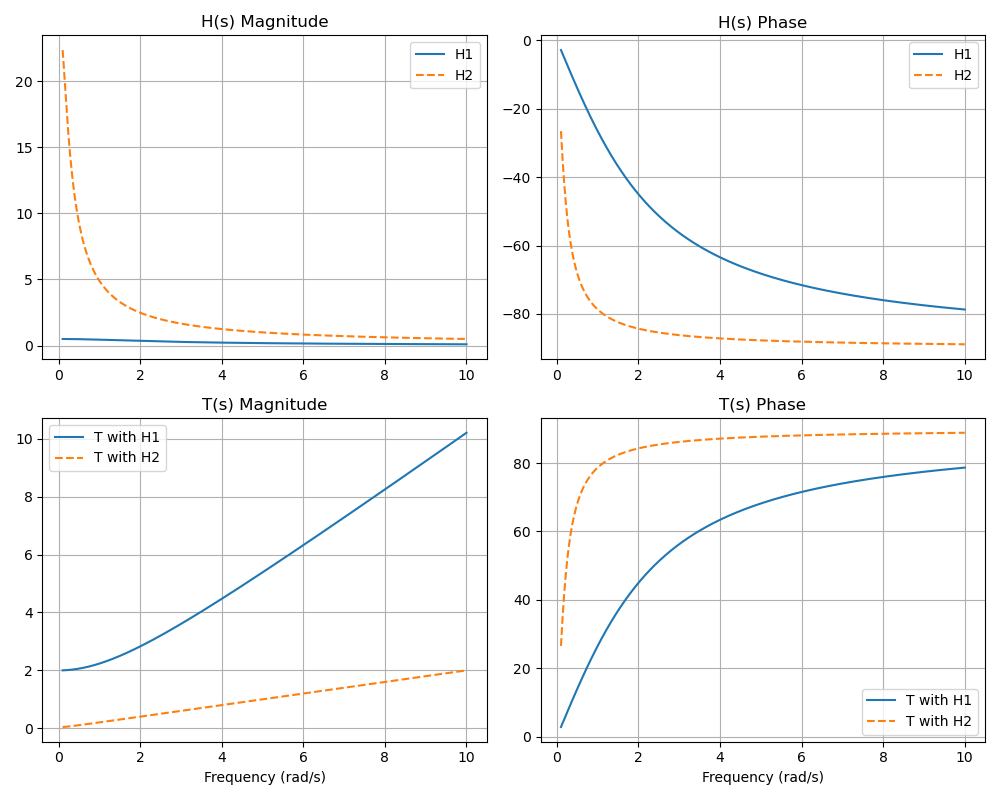
\includegraphics[width=0.75\linewidth]{Figure_h.png}
        \caption{H(s) is changing}
        \label{fig:placeholder}
    \end{figure}
\end{frame}
\begin{frame}{Plot with G(s) changing}
\begin{figure}
    \centering
    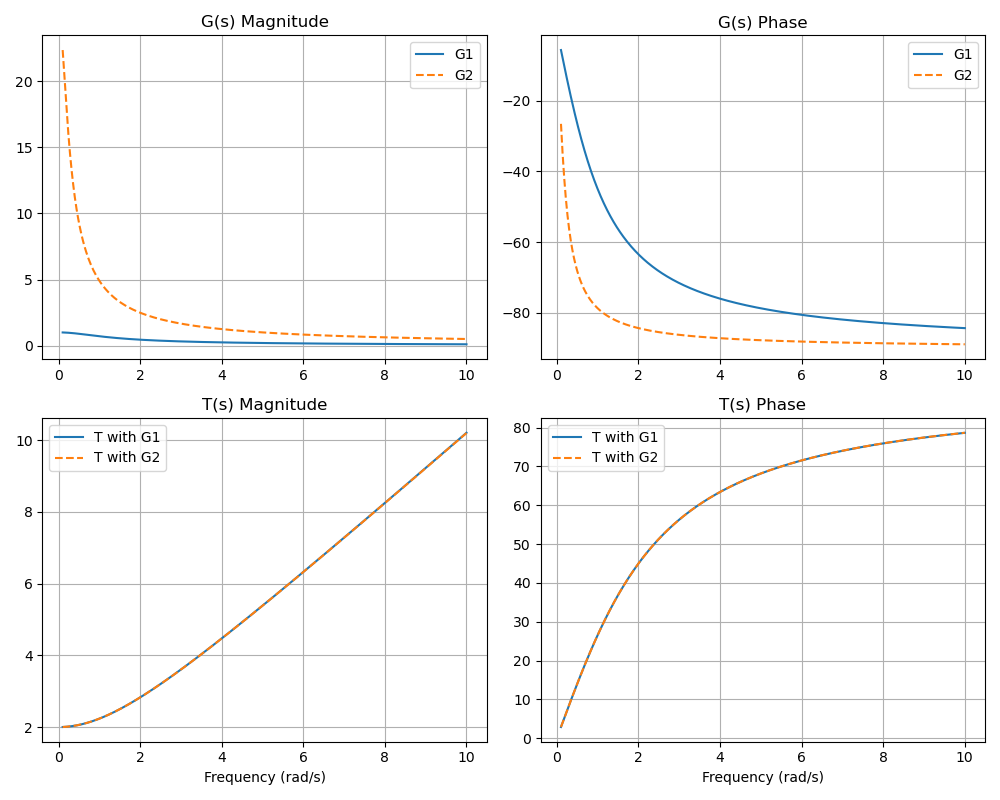
\includegraphics[width=0.75\linewidth]{Figure_g.png}
    \caption{G(s) Changing}
    \label{fig:placeholder}
\end{figure}
\end{frame}
 \end{document}